\documentclass[11pt,letterpaper]{article}
\usepackage[lmargin=1in,rmargin=1in,tmargin=1in,bmargin=1in]{geometry}
\usepackage{../style/homework}
\usepackage{../style/commands}
\setbool{quotetype}{true} % True: Side; False: Under
\setbool{hideans}{true} % Student: True; Instructor: False

% -------------------
% Content
% -------------------
\begin{document}

\homework{1: Due 02/13 (14)}{In learning you will teach, and in teaching you will learn.}{Phil Collins}

% Problem 1
\problem{10} Let $\mathcal{U}= \{ -10, -9, \ldots, 9, 10 \}$. Define the following subsets of $\mathcal{U}$:
	\[
	\begin{aligned}
	A&= \{ -2, 0, 5, 10 \} \\
	B&= \text{even numbers in } \mathcal{U} \\
	C&= \{ -9, -7, -5, -3, -1, 1, 3, 5, 7, 9 \} \\
	D&= \text{positive prime numbers in } \mathcal{U} \\
	E&= \{ -5, -4, \ldots, 4, 5 \} 
	\end{aligned}
	\]
Using the sets defined above, answer the following: 
        \begin{enumerate}[(a)]
        \item $A \cap B$
        \item $B \cup E$
        \item $E - A$
        \item $B^c$
        \item $|D|$
        \end{enumerate}



\newpage



% Problem 2
\problem{10} Define the following sets:
	\[
	\begin{aligned}
	A&= \text{set of multiples of 3} \\
	B&= \text{set of divisors of 30} \\
	C&= \text{set of even numbers less than 10} 
	\end{aligned}
	\]
Using the sets defined above, answer the following:
        \begin{enumerate}[(a)]
        \item List the elements of $B$.
        \item Give the largest element of $A$ less than 50 and the largest negative element of $A$.
        \item What are the elements of $B - A$?
        \item What are the elements of $A \cap B$?
        \item Are $B$ and $C$ disjoint? Explain. 
        \end{enumerate}



\newpage



% Problem 3
\problem{10} Look at the Venn diagram given below:
	\[
	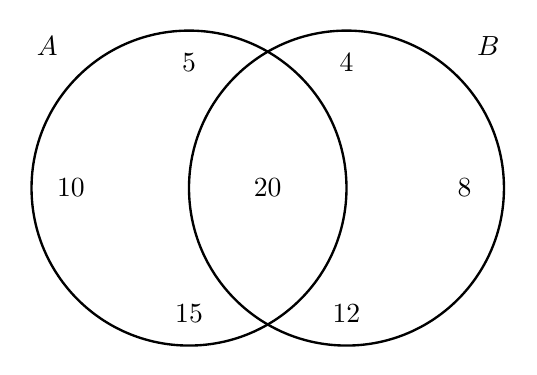
\begin{tikzpicture}
	\draw[line width=0.03cm] (-1,0) circle (2);
	\draw[line width=0.03cm] (1,0) circle (2);
	\node at (-2.8,1.8) {$A$}; 
	\node at (-1,1.6) {$5$}; \node at (-2.5,0) {$10$}; \node at (-1,-1.6) {$15$};
	\node at (2.8,1.8) {$B$};
	\node at (1,1.6) {$4$}; \node at (2.5,0) {$8$}; \node at (1,-1.6) {$12$};
	\node at (0,0) {$20$};
	\end{tikzpicture}
	\]
Use this diagram to answer the following:
	\begin{enumerate}[(a)]
	\item Assuming only a few of the elements of $A$ and $B$ are given in the diagram above, describe what the sets $A$ and $B$ likely represent.
	\item Place the numbers $25$, $16$, and $40$ in appropriate places in the given Venn diagram. 
	\item Using words, explain what numbers go in the same region of the Venn diagram in which $20$ is found.
	\item Using words, explain what numbers go in the same region of the Venn diagram in which $4$, $8$, and $12$ are found.
	\item What numbers would be placed outside of both the regions $A$ and $B$? Give an example.  
	\end{enumerate}



\newpage



% Problem 4
\problem{10} You are working with a student named Lucy. You give her the following sets: $A= \{ a, b, c, d, a \}$ and $B= \{ c, d, e, f \}$. 
	\begin{enumerate}[(a)]
	\item Lucy states that the cardinality of $A$ is 5. Explain why Lucy is wrong. How might you correct her?
	\item You ask Lucy to find $A \cup B$ and she states that this is $\{ c, d \}$. What has Lucy done wrong?
	\item Cameron overhears Lucy's answer in (b) and shouts that the answer is $\{ a, b, e, f \}$. How has Cameron misunderstood the mathematical word \textit{or} in this context? 
	\item Both Lucy and Cameron state that you cannot find $A - B$ because they are filled with letters and you cannot subtract letters. Explain what they have misunderstood about sets. 
	\end{enumerate}


\end{document}